\section{Main Results}

\subsection{Settings}

\subsubsection{Bandit}

We first analyze the standard bandit setting, i.e., $n = 1$ , and then generalize the results to many state dependent bandits setting. For simplicity, assume the reward $\rvr \in \sR^h$ is a deterministic vector. Using concentration the results can be generalized to random reward vectors, therefore recovering the stochastic bandit setting. Also we assume $r_k \in [0, 1]$, $\forall k \in [h]$.

In this setting, we use the NN policy to pull one arm $A_t \in [h]$ in each time step $t$, then observe the reward $r_{A_t}$. The policy net then uses the reward to update its weight vectors, using policy gradient method. After such $T$ steps, we are concerned with the regret,
\begin{equation*}
    \ell \triangleq \regret(\rvpi) \triangleq \r^{\max} \cdot T - \sum\limits_{t=0}^{T-1}{ \rvpi(t)^\top \rvr } = \sum\limits_{t=0}^{T-1}{ \rvpi(t)^\top \rvtilder }
\end{equation*}

\subsubsection{Episodic MDP}

In the Episodic MDP setting, in each time step, we use NN policy to take one action $A_t$, then observe a reward $R_{t+1}$ and next state $S_{t+1}$. After such $H$ steps, there is an ending state, and this trajectory terminates. Since we use policy gradient method (no value learning method here), the policy updates its weights using the cumulative reward collected from each trajectory. 


\subsection{Policy Gradient Method}

\begin{algorithm}[h]
   \caption{Policy Gradient Method Mixed with Uniform Exploration}
\label{alg:policy_gradient_uniform_exploration}
\begin{algorithmic}
   \STATE {\bfseries Input:} state feature vectors $\rvs_i$
   \STATE Initialize $\rvw_r \sim \gN\left( 0, \sigma \cdot \rmI \right)$, $\forall r \in [m]$, $\rva_k \sim \gN(0, \rmI)$, $\forall k \in [h]$.
   \FOR{$t=0$ {\bfseries to} $T-1$}
   \IF{$t < \sqrt{T}$}
   \STATE Uniformly randomly take action $A_{i,t}$. 
   \STATE Observe reward and next state.
   \ELSE
   \STATE Take action $A_{i,t} \sim \rvpi_{i}\left(\cdot \middle| S_{i,t} \right)$. 
   \ENDIF
   \STATE $\rvw_r(t+1) = \rvw_r(t) - \eta \cdot \frac{d\ell}{d \rvw_r(t)}$, $\forall r \in [m]$.
   \ENDFOR
\end{algorithmic}
\end{algorithm}

The objective of our analysis is the policy gradient method, mixed with uniform exploration, as shown in shown in \cref{alg:policy_gradient_uniform_exploration}. The reason why we need exploration will be explained later on, and technically it seems cannot be eliminated.

The policy gradient method works as follows. After initialization, the policy net $\rvpi$ will be updated using policy gradient calculated from collected reward. In the first $\sqrt{T}$ steps, actions are selected up to an uniform distribution over all actions. After that the NN policy $\rvpi$ is used to select actions.

\subsection{Main Results}




Tables contain textual material, whereas figures contain graphical material.
Specify the contents of each row and column in the table's topmost
row. Again, you may float tables to a column's top or bottom, and set
wide tables across both columns. Place two-column tables at the
top or bottom of the page.

\subsection{Citations and References}

Citations within the text should include the authors' last names and
year. If the authors' names are included in the sentence, place only
the year in parentheses, for example when referencing Arthur Samuel's
pioneering work \yrcite{Samuel59}. Otherwise place the entire
reference in parentheses with the authors and year separated by a
comma \cite{Samuel59}. List multiple references separated by
semicolons \cite{kearns89,Samuel59,mitchell80}. Use the `et~al.'
construct only for citations with three or more authors or after
listing all authors to a publication in an earlier reference \cite{MachineLearningI}.

Authors should cite their own work in the third person
in the initial version of their paper submitted for blind review.
Please refer to Section~\ref{author info} for detailed instructions on how to
cite your own papers.

Use an unnumbered first-level section heading for the references, and use a
hanging indent style, with the first line of the reference flush against the
left margin and subsequent lines indented by 10 points. The references at the
end of this document give examples for journal articles \cite{Samuel59},
conference publications \cite{langley00}, book chapters \cite{Newell81}, books
\cite{DudaHart2nd}, edited volumes \cite{MachineLearningI}, technical reports
\cite{mitchell80}, and dissertations \cite{kearns89}.


\if0
% In the unusual situation where you want a paper to appear in the
% references without citing it in the main text, use \nocite
\nocite{langley00}
\fi

\if0
\begin{table}[t]
\caption{Classification accuracies for naive Bayes and flexible
Bayes on various data sets.}
\label{sample-table}
\vskip 0.15in
\begin{center}
\begin{small}
\begin{sc}
\begin{tabular}{lcccr}
\toprule
Data set & Naive & Flexible & Better? \\
\midrule
Breast    & 95.9$\pm$ 0.2& 96.7$\pm$ 0.2& $\surd$ \\
Cleveland & 83.3$\pm$ 0.6& 80.0$\pm$ 0.6& $\times$\\
Glass2    & 61.9$\pm$ 1.4& 83.8$\pm$ 0.7& $\surd$ \\
Credit    & 74.8$\pm$ 0.5& 78.3$\pm$ 0.6&         \\
Horse     & 73.3$\pm$ 0.9& 69.7$\pm$ 1.0& $\times$\\
Meta      & 67.1$\pm$ 0.6& 76.5$\pm$ 0.5& $\surd$ \\
Pima      & 75.1$\pm$ 0.6& 73.9$\pm$ 0.5&         \\
Vehicle   & 44.9$\pm$ 0.6& 61.5$\pm$ 0.4& $\surd$ \\
\bottomrule
\end{tabular}
\end{sc}
\end{small}
\end{center}
\vskip -0.1in
\end{table}
\fi

\if0
\begin{figure}[ht]
\vskip 0.2in
\begin{center}
\centerline{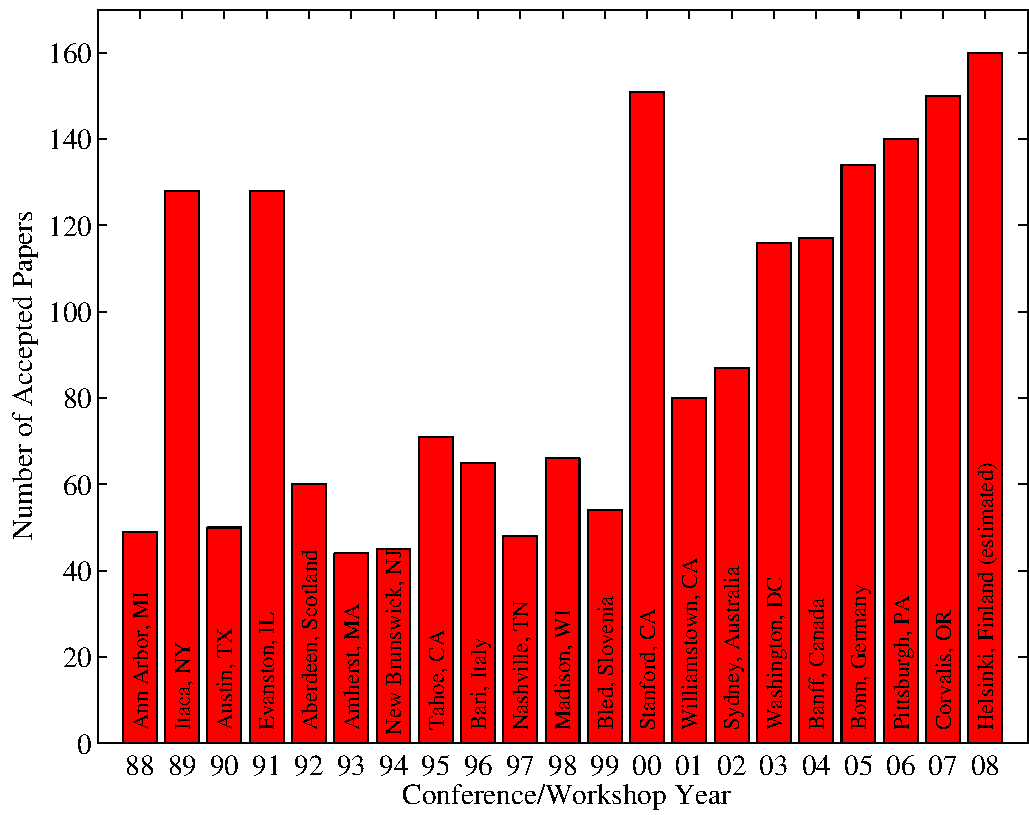
\includegraphics[width=\columnwidth]{icml_numpapers}}
\caption{Historical locations and number of accepted papers for International
Machine Learning Conferences (ICML 1993 -- ICML 2008) and International
Workshops on Machine Learning (ML 1988 -- ML 1992). At the time this figure was
produced, the number of accepted papers for ICML 2008 was unknown and instead
estimated.}
\label{icml-historical}
\end{center}
\vskip -0.2in
\end{figure}
\fi